\documentclass[report2]{subfiles}

\begin{document}
\section{Circuit Testing}
The keyboard encoder was tested twice. Once using a vhdl testbench that walked through cases, and once using the Altera FPGA board. Both rounds of testing were successful. \\
\subsection{VHDL Testbench}
The VHDL testbench ran through all 64 of the simple cases. \\
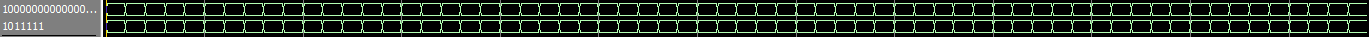
\includegraphics[width=\textwidth]{keyboard_full_test}
The multiple key cases were not tested, as those had been covered in tests for the 64 to 6 encoder circuit used as a component in the keyboard encoder. \\
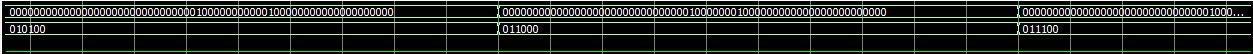
\includegraphics[width=\textwidth]{64_6_spec_test}
\subsection{Altera FPGA Board}
The circuit was also tested on the Altera De1-SOC board. To do so, the output of the encoder was put through an ascii code to 7 segment display decoder. This converted a subset of characters to the necessary codes for displaying characters. Switches on the FPGA board were linked to single key inputs, and a 7 segment display on the board was used to verify that the correct codes were being displayed. \\


\end{document}